To estimate the impact of beaver reintroduction on agricultural land use, I obtain data on (1) the Tayside beaver expansion from three comprehensive regional surveys conducted over a decade, (2) high-resolution satellite-derived land use classifications, (3) soil data on agricultural land compatibility, (4) satellite-derived elevation and slope data, and (5) river level from a network of in-situ hydrometry monitors across Scotland. To measure the impacts of beaver entry on agriculture, I employ the land use data, exploiting its spatiotemporal variation, spanning pre- and post-beaver entry periods, to test for land use change. To detect physical environment changes following beaver entry, I use the hydrometry data. In robustness checks, I use high-resolution data on soil type, elevation, and slope to run models on subsamples varying beaver habitat suitability. In all analyses, the unit of observation is a 1km$^2$ cell in a grid constructed by tessellating the study region in Fig. \ref{fig:study-area}. Subsamples of only ``river'' cells rely on a watercourse layer sourced from Ordnance Survey OpenData (CITE?).

\subsection{Beaver Expansion}
To 
\begin{itemize}
    \item Describe survey methods, with attention to causal inference concerns
    \item Describe how to translate survey observations to population estimates
\end{itemize}

\begin{figure}
    \centering
    \caption{Beaver Expansion}
    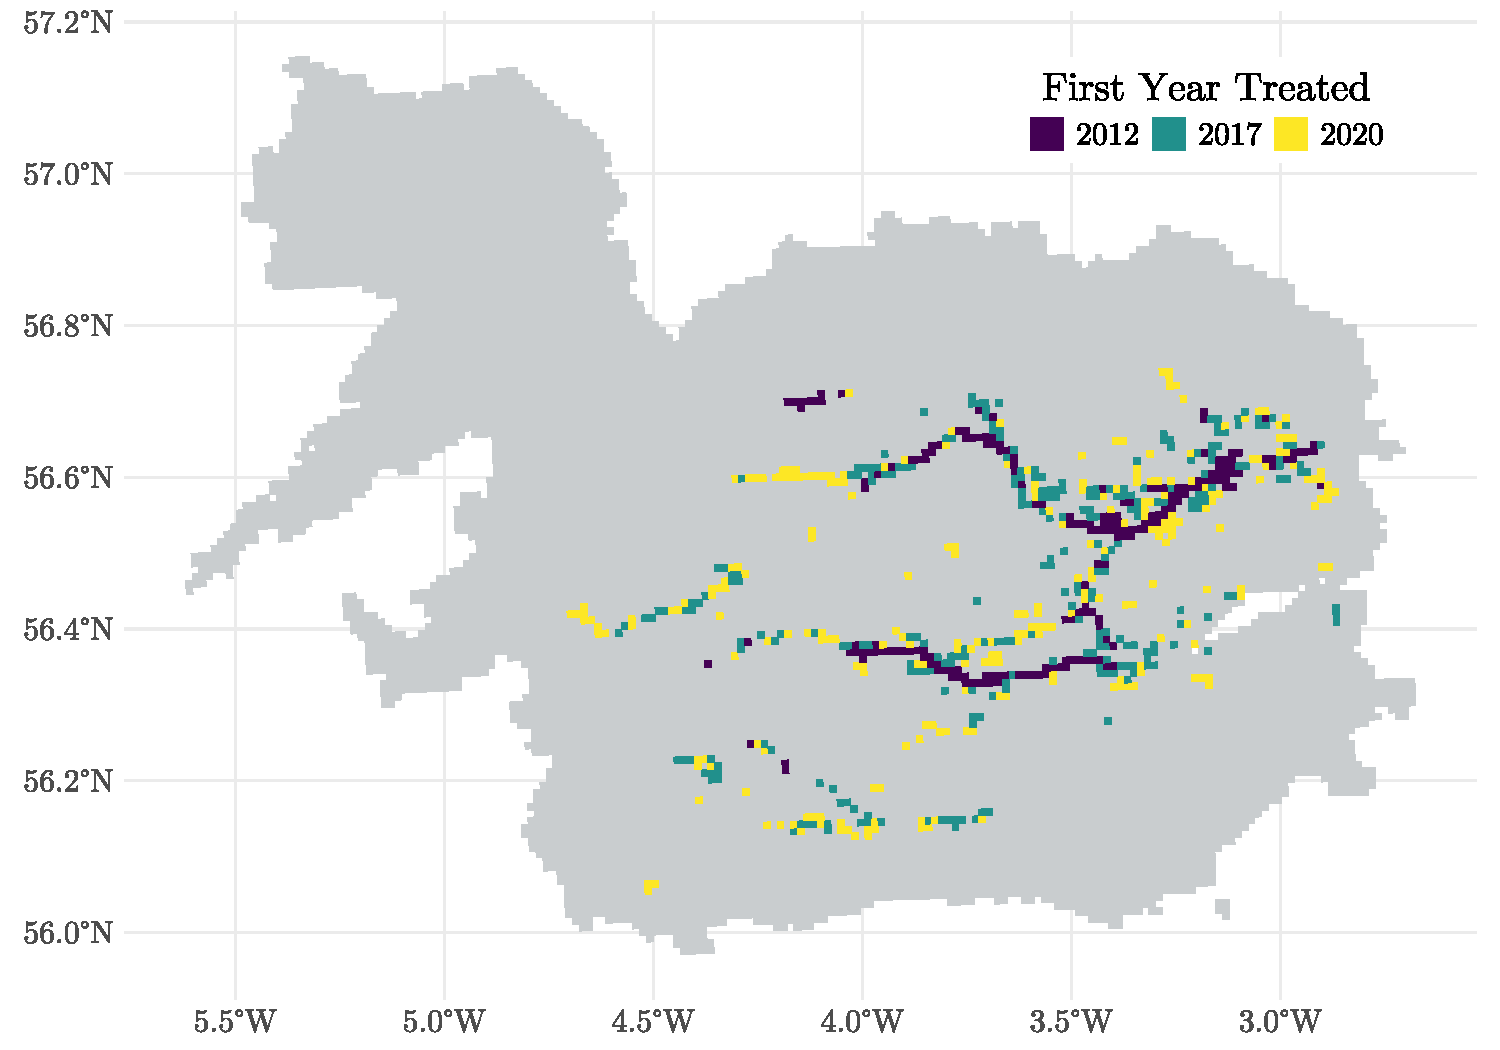
\includegraphics[width=0.7\linewidth]{output/figures/beaver_first_year_treated.pdf}
    \label{fig:enter-label}
    \caption*{\justifying \footnotesize Notes: Beaver detection by survey year in study region. Observation units are 1km$^2$ landscape grid cells. Data source: NatureScot and affiliated data procurement contractors. See main text for details.}
\end{figure}

\subsection{Land Cover Maps}
To capture spatiotemporal variation in agricultural land use, I employ the UK Center for Ecology \& Hydrology's repeated Land Cover Map product (LCM) at 25m resolution, which exists for 1990, 2000, 2007, 2015, 2017, 2018, 2019, 2020, 2021, and 2022. The LCM covers the entirety of Great Britain and North Ireland, deriving its classifications from Sentinel-2 seasonal 10-band composite image patches (CITE UKCEH LCM 2022 docs), with additional context layers on height, aspect, slope, distance to built structures and water bodies, foreshore, and woodland to ejudicate spectral confusion. Modern UKCEH models (since around 2015) classify 10m pixels into 21 land use classes, based on the Biodiversity Action Plan Broad Habitats (CITE Jackson et al 2000), using a random forest. As ground truth, UKCEH uses pixels classified in previous years with high accuracy (>80\%) and no observed change over three consecutive years. Predictions made on 10m pixels are then aggregated to land parcels and from there rasterized at 25m resolution. I consider agricultural any pixel classified as ``arable'' in the UKCEH LCM, which includes cropped and freshly ploughed land (Fig. \ref{fig:ukceh-lcm-raw}). I do not include the closely related class of ``improved grassland'' due to its low recall and precision (74.3\% and 91.1\%, respectively) compared to ``arable,'' which has the highest recall and second highest precision of any class (97.6\% and 92.7\%, respectively), when validated on a set of reference points sourced from countryside surveys, National Forest Inventory, Rural Payment Agency, manual Sentinel-2 image interpretation, and UKCEH field collection.\footnote{This is largely due to the difficulty of differentiating between grassland types, including improved, neutral, calcereous, and acid, which exist on a spectral continuum.} Nearly all false negative arable pixels were mislabeled as improved grassland (93.4\%). Similarly, the majority of false positive arable-classified pixels were in fact improved grassland (55.8\%). I aggregate the 25m ``arable'' mask up to the 1km$^2$ grid cells to produce a measure on the unit interval of agricultural land share, weighting by overlap proportion for raster cells not entirely contained within the 1km$^2$ landscape cell (Fig. \ref{fig:ukceh-lcm-agg}). 

\begin{figure}
    \centering
    \caption{Agricultural land use}
    \begin{subfigure}{0.39\linewidth}
        \caption{\centering 25m raster cells classified as agriculture}
        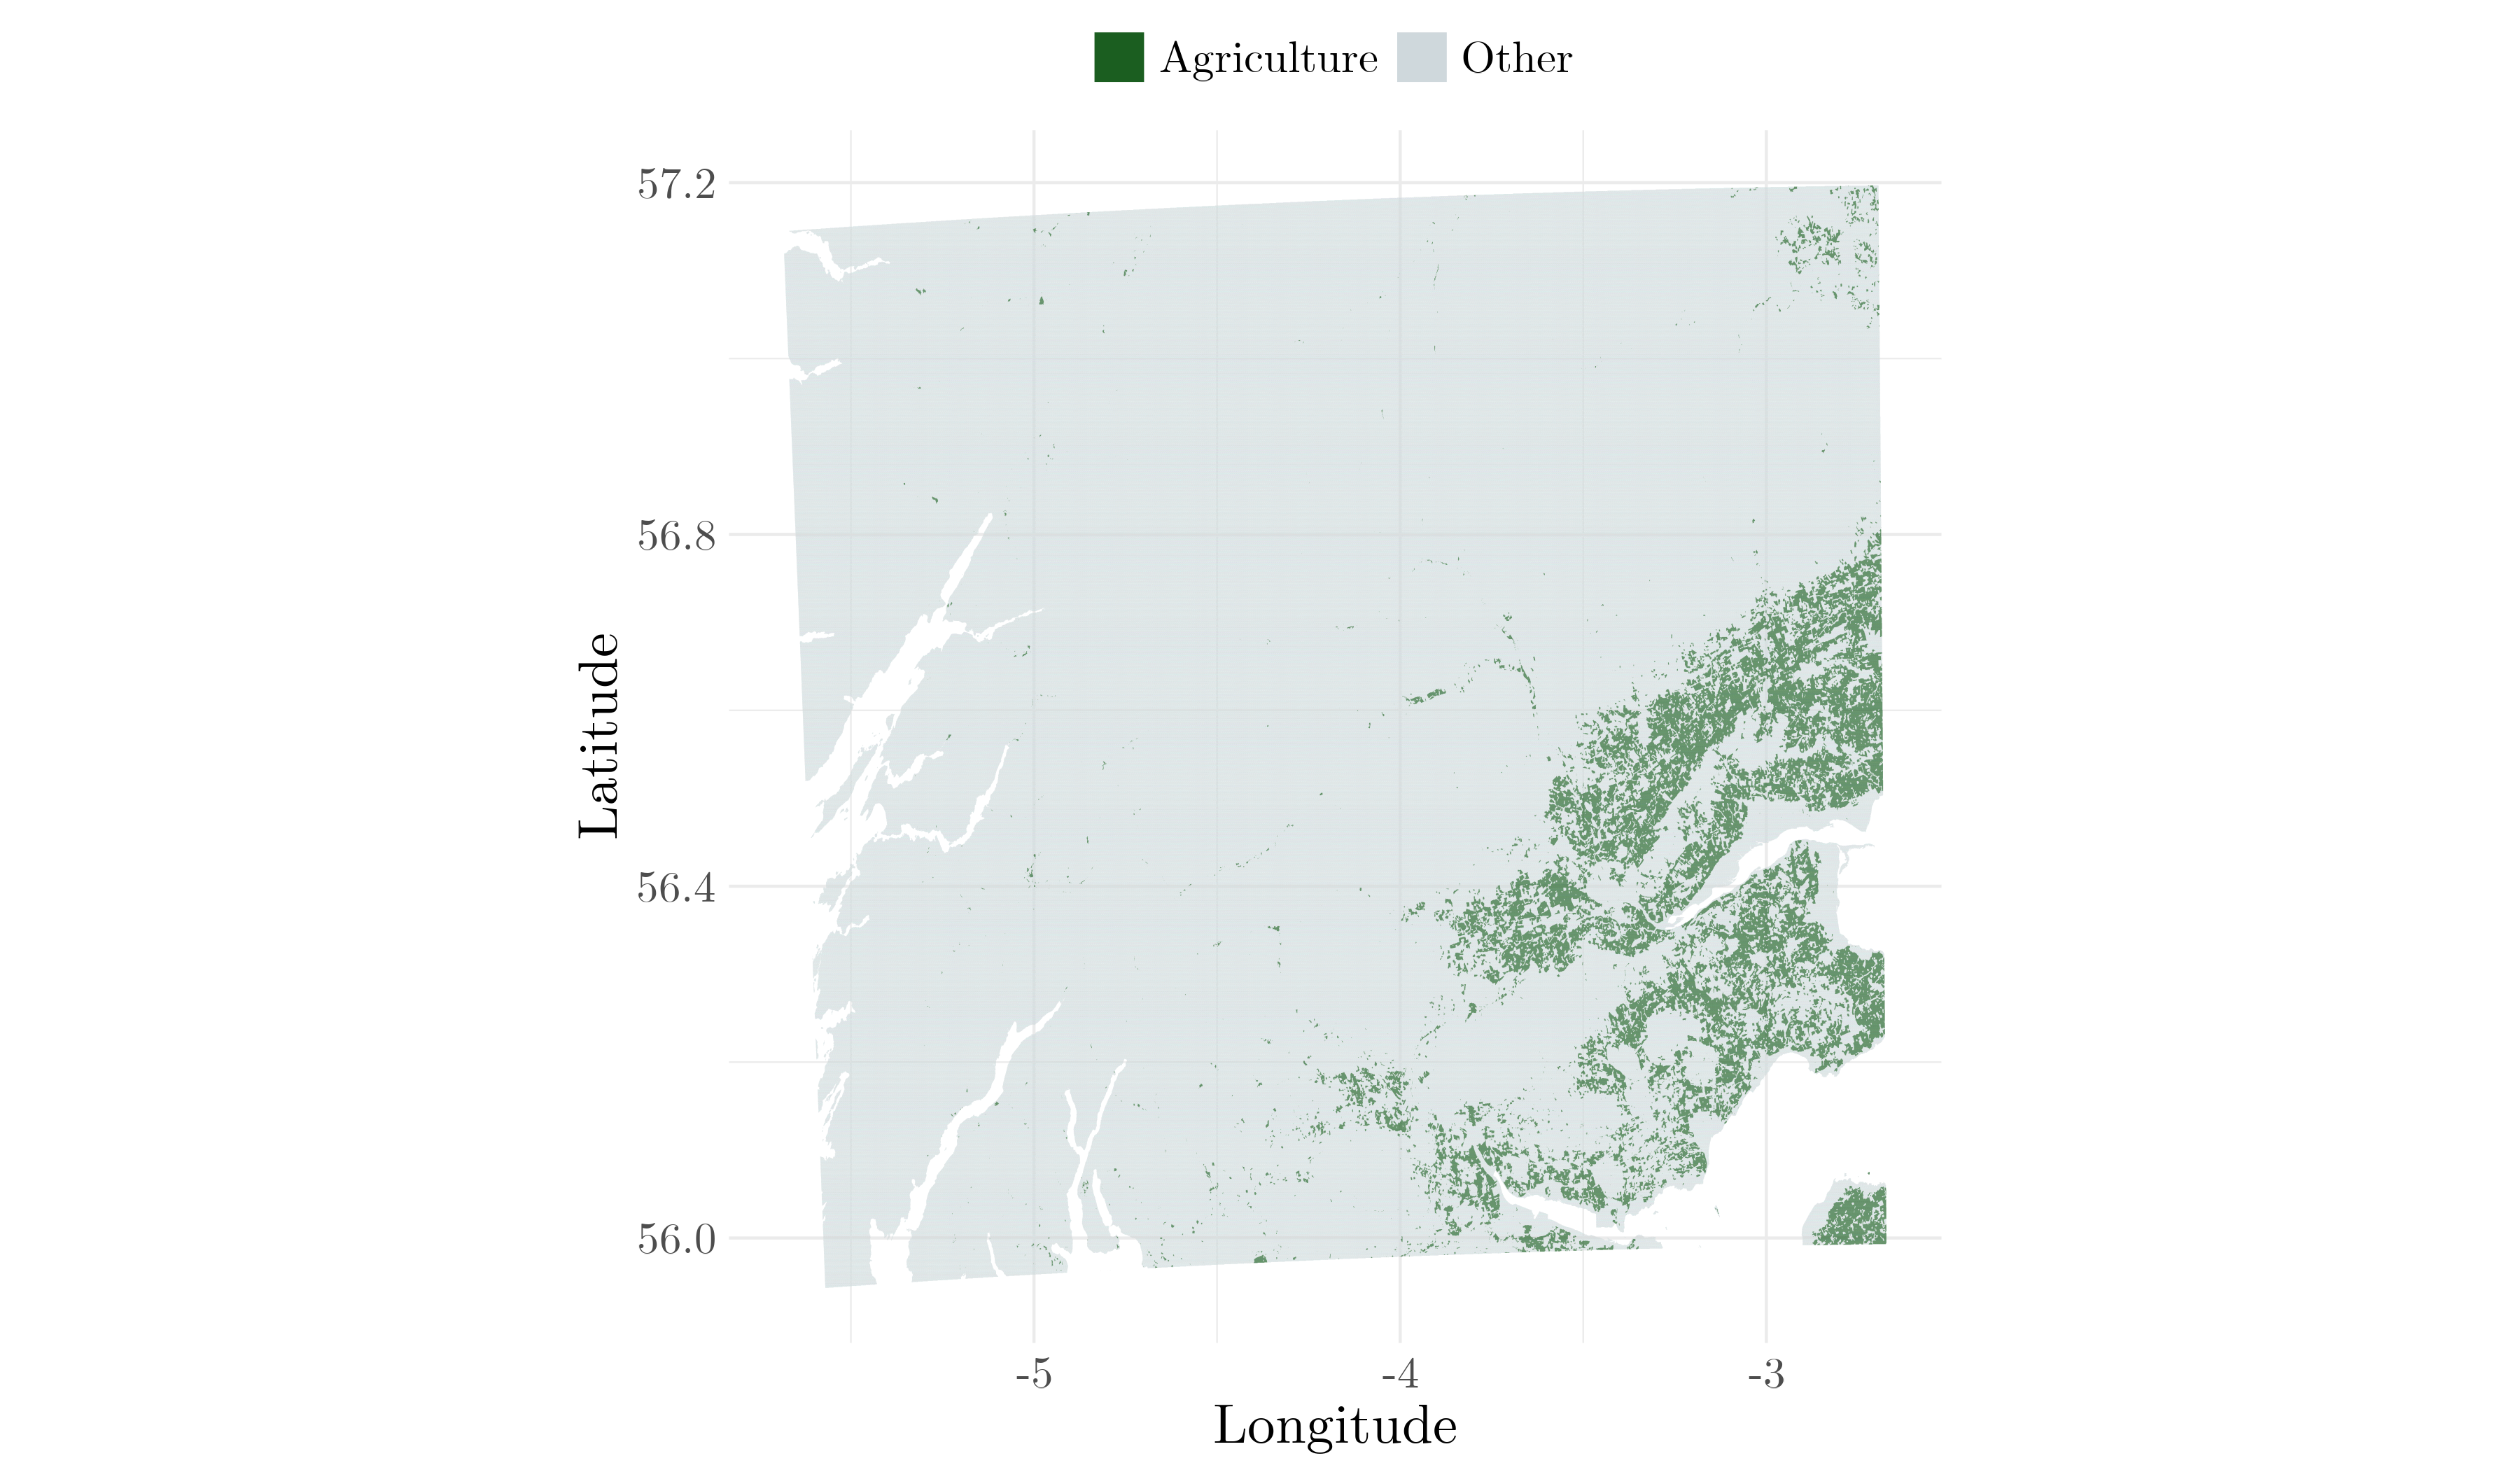
\includegraphics[width=\linewidth]{output/figures/lcm_in_study_area.png}
        \label{fig:ukceh-lcm-raw}    
    \end{subfigure}
    \begin{subfigure}{0.58\linewidth}
        \caption{\centering Agricultural raster layer aggregated to 1km$^2$ landscape grid cells}    
        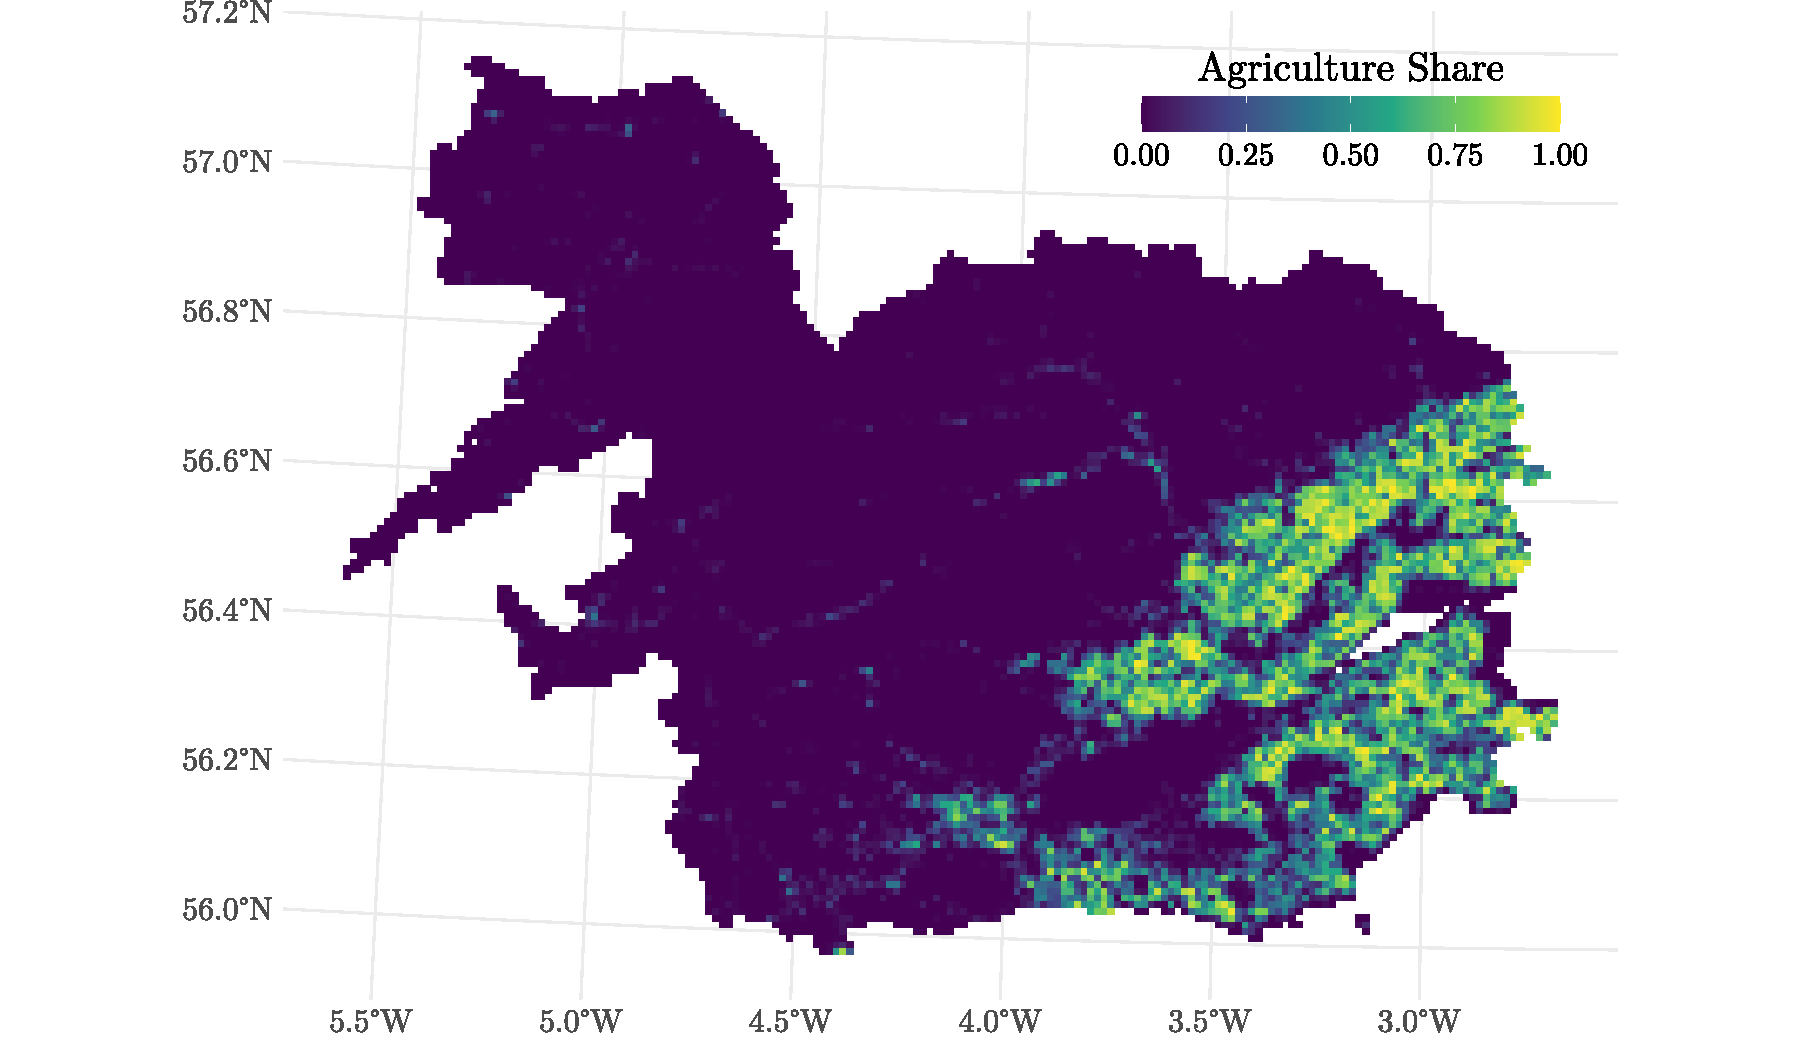
\includegraphics[width=\linewidth]{output/figures/lcm_agg_river_grid.pdf}
        \label{fig:ukceh-lcm-agg}
    \end{subfigure}
    \caption*{\justifying \footnotesize Notes: Data from the UK Center for Ecology \& Hydrology Land Cover Map (25m rasterized land parcels, GB). 2022 data used for illustration. See main text for details.}
\end{figure}

\subsection{River}
\begin{itemize}
    \item Describe hydrometry network and history
    \item Describe measurements collected, with special attention to the interpretation of river level
\end{itemize}

\subsection{Landscape characteristics}

Briefly describe: 

\begin{itemize}
    \item Soil (constant)
    \item Elevation from ASTER (https://lpdaac.usgs.gov/products/astgtmv003/)  (constant)
    \item Slope calculated as first derivative of elevation (constant)
    \item Temperature, precip, and leaf area index from ERA5 (time varying)
\end{itemize}

% \subsection{Remote Sensing of Floods}